\documentclass{standalone}
\usepackage{tikz}

\begin{document}

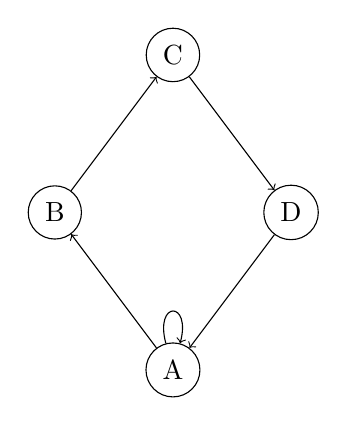
\begin{tikzpicture}
    \node[shape=circle,draw=black] (A) at (0,0) {A};
    \node[shape=circle,draw=black] (B) at (-1.5,2) {B};
    \node[shape=circle,draw=black] (C) at (0,4) {C};
    \node[shape=circle,draw=black] (D) at (1.5,2) {D};

    \path [->] (A) edge node[below] {} (B);
    \path [->](B) edge node[below]  {} (C);
    \path [->](C) edge node[below]  {} (D);
    \path [->](D) edge node[below]  {} (A);
    \path[->] (A) edge[loop above, looseness=8] (A);
\end{tikzpicture}

\end{document}